\chapter{Turbomacchine assiali}

\section{Generalità}
Si possono seguire diversi approcci via via più raffinati.

Nell'approccio monocimensionale il flusso è rappresentato da un unico tubo di corrente con condizioni di deflusso mediate. Risulta utile in fase di pre dimensionamento. 

Nell'approccio bidimensionale/quasi-tridimensionale il flusso è rappresentato da più tubi di corrente con condizioni di deflusso mediate nella singola regione di deflusso. Si utilizza in fase di dimensionamento. Il piano su cui si va a considerare il fluido è il mantello cilindrico che compone la macchina, aperto a piano. Si analizza l'equilibrio radiale del flusso della macchina. Ho delle corone cilindriche che attraverso la macchina che scambiano energia e impogno l'equilibrio radialmente. 

L'approccio tridimensionale si usa in fase di ottimizzazione per tenere conto dei flussi secondari. Questo è un approccio computazionalmente molto oneroso.

Si andrà quindi ad approfondire il secondo approccio.

\section{Nomenclatura}
\begin{figure}[h!]
\centering
\begin{minipage}{.5\textwidth}
  \centering
  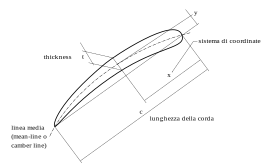
\includegraphics[width=.9\linewidth]{fig/profiloDef.pdf}
  \captionof{figure}{}
  \label{}
\end{minipage}%
\begin{minipage}{.5\textwidth}
  \centering
  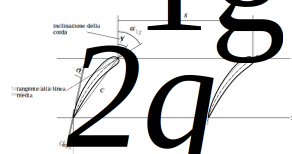
\includegraphics[width=.9\linewidth]{fig/schiera_2.pdf}
  \captionof{figure}{}
  \label{}
\end{minipage}
\end{figure}

Per il profilo isolato posso definire le seguenti grandezze adimensionali:
\begin{align*}
\cfrac{x}{c} \;\;\; \cfrac{y}{c} \;\;\; \cfrac{t}{c}
\end{align*}
Posso poi definire la solidità della schiera come segue:
\begin{equation}
\sigma = \cfrac{c}{s}
\end{equation}

\subsection{Definizioni geometriche}
$\theta$: deflessione geometrica del profilo (angolo di Camber);\\
$\gamma$: ancolo di calettamento del profilo della schiera (inclinazione della corda rispetto alla direzione ortogonale);\\
$\alpha_{1g}, \alpha_{2g}$: inclinazioni delle tangenti alla linea media rispetto alla direzione ortogonale.
\begin{align*}
\theta = \alpha_{1g} - \alpha_{2g} = \Delta \alpha_{g}
\end{align*}

\subsection{Definizioni per la corrente fluida}
$\alpha_1$: inclinazione del vettore velocità rispetto alla direzione di riferimento ortogonale alla schiera, una palettatura non riuscirà mai a deviare la corrente tanto quanto è inclinata geometricamente;\\
$\alpha$: inclinazione del vettore velocità con riferimento alla corda (angolo di attacco del flusso rispetto la schiera);\\
$i$: inclinazione del vettore velocità rispetto la tangente alla linea media (angolo di incidenza);\\
$\delta$: angolo di deviazione o deviazione (angolo di deviazione del flusso in uscita rispetto la tangente alla linea media);\\
$\epsilon = \Delta \alpha$: entità della deflessione subita dal flusso tra ingresso e uscita.
\begin{figure}
\centering
  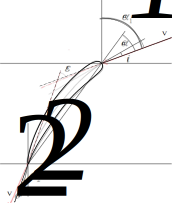
\includegraphics[width=.35\textwidth]{fig/palasing.pdf}
\caption{}
\label{fig:palasing}
\end{figure}
Nel caso delle turbine le deviazioni sono più alte rispetto ai compressori, rallentare una corrente è sempre molto più facile che accelerarla. 

Dalle considerazioni geometriche viste prima si può scrivere
\begin{equation}
\epsilon = \theta + i - \delta
\end{equation}

\subsection{Forze}
Le forze agenti sulla schiera di pale posso scriverle rispetto al sistema di rif assiale tangenziale per determinare la coppia, ovvero la potenza fornita all'albero nel caso di compressore. La componente assiale sarà la spinta che i cuscinetti dovranno sopportare per il funzionamento ma ri riperquotono anche sulle perdite di carico. 

Le forze vanno anche declinate sotto il profilo di portanza e resistenza. Si tratta delle stesse forze su due sistemi di riferimento diversi. 

\begin{align*}
	\begin{cases}
		F_a = f(\Delta v, \Delta p_0)\\
		F_t = f(\Delta v, \Delta p_0)
	\end{cases}
\end{align*}
\begin{align*}
	\begin{cases}
		L = f(F_a,F_t)\\
		D = f(F_a,F_t)
	\end{cases}
\end{align*}

Considero una schiera palare e considero un volume di controllo ($ABCD$) che segue la linea media del profilo. Le velocità in ingresso e in uscita le scompongo nella direzioe assiale e radiale. 

\begin{figure}[h!]
\centering
\begin{minipage}{.4\textwidth}
  \centering
  \includegraphics[width=.85\linewidth]{fig/schiera1.pdf}
  \captionof{figure}{}
  \label{}
\end{minipage}%
\begin{minipage}{.6\textwidth}
  \centering
  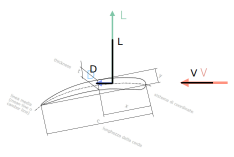
\includegraphics[width=.85\linewidth]{fig/LDref.pdf}
  \captionof{figure}{}
  \label{}
\end{minipage}
\end{figure}
Applico le equazioni di conservazione. Per continuità ho:
\begin{equation}
s \rho V_{1a} = s \rho V_{2a} \Rightarrow V_{1a} = V_{2a} = V_a
\end{equation}
Dove ho ipotizzato $\rho$ costante, per un compressore assiale i rapporti di compressione per stadio sono modesti, nel caso di una turbina non sarebbe valido. Per quanto riguarda la quantità di moto in direzione tangenziale:
\begin{equation}
F_t= \dot{m} \Delta V_t = s \rho	V_a (V_{1t}-V_{2t})
\end{equation}
In direzione assiale
\begin{equation}
F_a = s (p_1 - p_2)
\end{equation}

Scrivendo la pressione nelle componenti di pressione statica e dinamica posso espandere l'espressione delle forze assiali ottenendo:
\begin{equation}
F_a =\ldots=\cfrac{1}{2} \rho s (V_{t2}-V_{t1}) (V_{t2}+V_{t1}) + s \Delta p_0
\end{equation}

$\Delta p_0$ è la perdita di pressione totale, rappresenta quindi la perdita di carico nel deflusso attraverso la schiera. $(V_{t2}-V_{t1})$ rappresenta il trasferimento di quantità di moto. Se divido il termine $(V_{t2}+V_{t1})$ per $2$ ottengo l'espressione della velocità tangenziale all'infinito (velocità media indisturbata).
\begin{align*}
\cfrac{(V_{t2}+V_{t1})}{2} = V_{t \infty}
\end{align*}

Eseguendo ulteriori semplificazioni posso scrivere
\begin{equation}
F_a = -F_t \cfrac{V_{t \infty}}{V_a} + \Delta p_0 = - F_t \tan \alpha_{\infty} + s \Delta p_0
\end{equation}

Oltre a questa grandezza posso definire un coefficiente di perdita $y$ come
\begin{equation}
y = \cfrac{\Delta p_0}{p_{02}-p_2} = \cfrac{\Delta p_0}{\cfrac{1}{2} \rho V_2^2}
\end{equation}
Nota bene: è stato usato lo stesso simbolo ma non deve essere confuso con il nuemro di Camber.

Nel sistema di riferimento relativo, le forze vengono scomposte nella componente di \textit{Lift} (ortogonale alla velocità incidente) e nella componente di \textit{Drag} (parallela alla velocità incidente. 
\begin{figure}
\centering
  \includegraphics[width=.7\textwidth]{fig/triang1.pdf}
\caption{}
\label{fig:triang1}
\end{figure}
Posso quindi scrivere le espression di lift e drag e le forze nelle componeneti assiali:
\begin{equation}
	\begin{cases} 
		L = F_t \cos \alpha_{\infty} -  F_a \sin \alpha_{\infty}\\
		D = F_t \sin \alpha_{\infty} +  F_a \cos \alpha_{\infty}
	\end{cases}
\end{equation}
\begin{equation}
	\begin{cases} 
		L = L (\sin \alpha_{\infty} -  D \cos \alpha_{\infty})\\
		D = L \cos \alpha_{\infty} +  D \sin \alpha_{\infty}
	\end{cases}
\end{equation}

\subsection{Adimensionalizzazione delle forze}
Posso a questo punto definire $c_d$ e $c_L$:
\begin{equation}
c_L = \cfrac{L}{\cfrac{1}{2} \rho c V_{\infty}^2}
\end{equation}
\begin{equation}
c_D = \cfrac{D}{\cfrac{1}{2} \rho c V_{\infty}^2}
\end{equation}
Il coefficiente di forza $c_F$ sarà definito come:
\begin{align*}
c_F = \cfrac{F_t}{\cfrac{1}{2} \rho c V_{\infty}^2} = \cfrac{s V_a (V_{t1}-V{t2}=}{\cfrac{1}{2} c V_{\infty}^2} = ...
\end{align*}
\begin{figure}
\centering
  \includegraphics[width=.4\textwidth]{fig/trigrel.pdf}
\caption{}
\label{fig:trigrel}
\end{figure}
Usando le relazioni $V_a = V_{\infty} \cos \alpha_{\infty}$ e $V_{t1,2} = \tan \alpha_{1,2}$ (vedi Figura \ref{fig:trigrel}) si espande ulteriormente la relazione ottenendo
\begin{equation}
c_F = 2 \cfrac{s}{c} \cos ^ 2 (\alpha_{\infty})(\tan \alpha_1 - \tan \alpha_2)
\end{equation}

Allo stesso modo posso espandere $c_P$
\begin{equation}
c_P = \cfrac{F_a}{\cfrac{1}{2} \rho c V_{\infty}^2} = \cfrac{s \Delta p_0 - F_t \tan \alpha_{\infty}}{\cfrac{1}{2} \rho c V_{\infty}^2} = \cfrac{s \Delta p_0}{\cfrac{1}{2} \rho c V_{\infty}^2} - c_F \tan \alpha_{\infty}
\end{equation}
Ricordando la relazione del coefficiente di perdita
\begin{align*}
t = \cfrac{\Delta p_0}{\cfrac{1}{2} \rho c V_2^2}
\end{align*}
Posso scrivere
\begin{align*}
c_P = \left(\cfrac{s}{c}\right)y \left(\cfrac{V_2}{V_{\infty}}\right)^2 - c_F \tan \alpha_{\infty}
\end{align*}
E quindi
\begin{equation}
c_P = \left(\cfrac{s}{c}\right)y \cfrac{\cos^2 \alpha_{\infty}}{\sin^2 \alpha_2} -2\left(\cfrac{s}{c}\right) \left(\tan \alpha_1 - \tan \alpha_2 \right) \sin \alpha_{\infty} \cdot cos \alpha_{\infty}
\end{equation}

Ho così ottenuto tutte le relazioni per passare da coefficienti di portanza e resistenza a coefficienti di forza e pressione.

Nel caso di fluido ideale non viscoso il drag è nullo, in questo caso allora il Lift sarà uguale a $2$ e dipenderà solo dalla geometria della schiera. 

Ipotesi di perdite nulle $\Delta p_0 = 0$
\begin{equation}
\begin{cases}
F_a = s \rho V_{\infty t} (V_{2t}-V{1t})\\
F_t = s \rho V_a (V_{1t}-V{2t})
\end{cases}
\end{equation}

Come ho fatto con le forze, posso esprimere quindi i coefficienti adimensionali secondo i diversi sistemi di coordinate. 

Posso trovare allora
\begin{equation}
\begin{cases}
c_L = c_F \cos \alpha_{\infty} - c_P \sin \alpha_{\infty} \\
c_D = c_F \sin \alpha_{\infty} + c_P \cos \alpha_{\infty}
\end{cases}
\end{equation}
Sostituendo $c_F$ e $c_P$ ottengo
\begin{equation}
\begin{cases}
c_L = 2 \cfrac{s}{c} (tan \alpha_1 - \tan \alpha_2) \cos \alpha_{\infty} - c_D \tan \alpha_{\infty} \\
c_D = \cfrac{s}{c} y \cfrac{cos^3 \alpha_{\infty}}{\cos \alpha_2}
\end{cases}
\end{equation}
Sotto le ipotesi di flusso a potenziale non c'è generazione di forze. Si introduce quindi una rotazione nel flusso per modellare matematicamente il profilo (teorema di Kutta-Jukowsky). In questo modo sull'estradosso la velocità sarà maggiore di $V_{\infty}$ mentre nell'intradosso sarà minore. Si calcola quindi la circuitazione. Con $L$ è indicata la forza, con $\Sigma$ la forza della circuitazione.
\begin{equation}
\Sigma = \oint \overline{v} \cdot d \overline{l} \;\;\; L = \rho \sigma V_{\infty}
\end{equation}

In questo modo, anche senza avere la precisione che si avrebbe in una simulazione fluidodinamica del profilo, riesco a modellare in maniera snella anche una schiera di pale. Avrò semplicemente l'integrale all'ingresso e all'uscita della schiera su un volume di controllo. 
\begin{figure}
\centering
\begin{minipage}{.3\textwidth}
  \centering
  \includegraphics[width=.95\linewidth]{fig/cdcl.pdf}
  \captionof{figure}{}
  \label{fig:cdcl}
\end{minipage}%
\begin{minipage}{.7\textwidth}
  \centering
  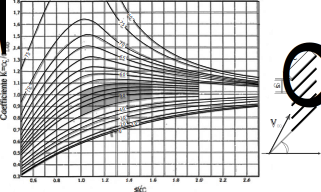
\includegraphics[width=.95\linewidth]{fig/EffSchiera.pdf}
  \captionof{figure}{}
  \label{fig:EffSchiera}
\end{minipage}
\end{figure}

Abbiamo poi la possibilità di correlare il comportamento del profilo isolato tra angolo di attacco e coefficienti di lift e di drag (Figura \ref{fig:cdcl}). Per quanto riguarda il $c_L$ si avrà una parte sostanzialmente lineare mentre il coefficiente di drag è via via crescente. Si arriva infine ad un punto di stallo. Le schiere lavorano nella parte lineare ma posso valutare le prestazioni tentando di correlare quello che succede su un profilo a quello che succede su una schera di assegnara solidità.

Statisticamente si diagramma anche cosa succede tra il rapporto coefficiente di lift e coefficiente di lift di profilo isolato e l'angolo di attacco rispetto al rapporto solidità su corda (Figura \ref{fig:EffSchiera}). 
Il range di solidità a quale si fa riferimento varia tra $1$ e$ 1.5 - 1.6$ non si va oltre a $2$. L'angolo di schiera è tra i $45 - 52 \; gradi$. In questo range il coefficiente $c_L / c_{L \infty}$ è molto vicino all'unità. 

In fase di progettazione si usano i dati del profilo isolato e si corregge il coefficiente secondo questi diagrammi. In contesto industriale si simula direttamente una schiera. 

\section{Ugelli e diffusori}
Le definizioni sono note e stranote.
\begin{figure}
\centering
\begin{minipage}{.5\textwidth}
  \centering
  \includegraphics[width=.6\linewidth]{fig/Ugello.pdf}
  \captionof{figure}{Ugello}
  \label{}
\end{minipage}%
\begin{minipage}{.5\textwidth}
  \centering
  \includegraphics[width=.6\linewidth]{fig/Diffusore.pdf}
  \captionof{figure}{Diffusore}
  \label{}
\end{minipage}
\end{figure}
Posso rappresentare queste trasformazioni sul piano $h-s$ con una trasformazione non isoentropica. 
\begin{equation}
\eta_{is} = \cfrac{h_{2s} - h_1}{h_2-h_1} = \cfrac{c_2^2 - c_1^2}{c_{2s}^2 - c_1^2}
\end{equation}
Nel caso di ugelli per $Ma < 0.3$ posso scrivermi tutte le grandezze
\begin{equation}
\begin{cases}
p_{01} = p_1 + \cfrac{1}{2} \rho c_1^2 \;\; \to  \;\; c_1^2 = \cfrac{2}{\rho} (p_{01} - p_1)\\
p_{02} = p_2 + \cfrac{1}{2} \rho c_{2s}^2 \;\; \to  \;\; c_{2s}^2 = \cfrac{2}{\rho} (p_{01} - p_1)\\
p_{02} = p_2 + \cfrac{1}{2} \rho c_2^2 \;\; \to  \;\; c_2^2 = \cfrac{2}{\rho} (p_{02} - p_2)
\end{cases}
\end{equation}
Sostituendo queste relazioni nell'espressione del rendimento si ottiene
\begin{equation}
\eta_{is} = \cfrac{p_{02} - p_2 - (p_{01} - p_1)}{p_{01} - p_2 - (p_{01} - p_1)}=\cfrac{p_{02} - p_2 -(p_{01} - p_1)}{p_1-p_2}=1- \cfrac{\Delta p_0}{p_1 - p_2}
\end{equation}

$\Delta p_0$ rappresenta la perdita tra ingresso e uscita. 

Per i diffusori si consideri sempre $Ma<0.3$ si possono usare le stesse espressioni, si ottiene un rendimento isoentropico come segue.
\begin{equation}
\eta_{is} = \cfrac{p_2 - p_1}{p_2-p_1 + (p_{01}-p_{02})} = \cfrac{c_1^2 - c_{2s}^2}{c_1^2 - c_2^2}
\end{equation}
L'utilizzo di un rendimento isoentropico è meno espressivo nel caso di un diffusore, ha maggior significato fisico un altra cosa, qual'è l'entita di $ \Delta p$ recuperabile della parte eccedente la pressione statica in ingresso.
\begin{equation}
\eta_{is} = \cfrac{p_{01} - p_1 - (p_{01} - p_2)}{p_{01} - p_1-(p_{02} - p_2)} = \cfrac{p_2 - p_1}{p_2 - p_1 + (p_{01} - p_{02})} = \cfrac{1}{1- \cfrac{\Delta p_0}{p_2 - p_1}}
\end{equation}
Definendo il coefficiente di recupero di pressione come
\begin{equation}
c_p = \cfrac{p_2 - p_1}{p_{01} - p_1}
\end{equation}
Cerchiamo però il legame tra coefficiente di recupero e rendimento isoentropico. Rimanipolando le formule si ottiene
\begin{equation}
\cfrac{1}{\eta_{is}} = \cfrac{p_2 - p_1 + (p_{01} - p_{02})}{p_2 - p_1} = \cfrac{p_{01} - p_1 - (p_{02} - p_2)}{p_2-p_1} = \cfrac{1}{c_P} - \cfrac{p_{02} - p_2}{p_2 - p_1}
\end{equation}

Posso definire un coefficiente di pressione ideale:
\begin{equation}
c_{pi} = \cfrac{p_2 - p_1 + (p_{01} - p_{02})}{p_{01} - p_1}
\end{equation}

Esprimendo secondo $A_1$ e $A_2$, aree di ingresso e uscita del diffusore 
\begin{equation}
c_{pi} = \cfrac{c_1^2 - c_2^2}{c_1^2} = 1 - \left( \cfrac{c_2}{c_1}\right)^2 = 1- \left(\cfrac{A_1}{A_2} \right)^2 =1-\cfrac{1}{A_R^2}
\end{equation}

A questo punto ottengo un rapporto
\begin{equation}
\cfrac{c_P}{c_{pi}} = ... = \eta_{is}
\end{equation}

Il diffusore funziona bene finchè il rapporto tra sezione di uscita e sezione di ingresso è molto piccolo. 
\begin{figure}
\centering
  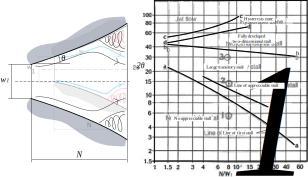
\includegraphics[width=.7\textwidth]{fig/stallo.pdf}
\caption{Zone di stallo}
\label{fig:stallo}
\end{figure}
\begin{figure}
\centering
  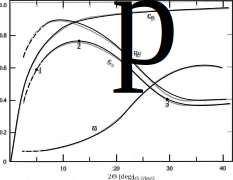
\includegraphics[width=.5\textwidth]{fig/DiffPerf.pdf}
\caption{Tipiche curve di performance per un diffusore bidimensionale con $L/W_1 = 0.8$}
\label{fig:DiffPerf}
\end{figure}
In figura sono rappresentate le tipiche curve di un diffusore.

\section{Schiere palari}
Le schiere di pale possono essere di espansione, in cui si ha un'accelerazione del flusso e quindi un comportamento simile ad un ugello. Nelle schiere di compressione si ha invece una trasformazione della velocità in pressione. 

\subsection{Schiere di espansione}
Il rendimento isoentropico di queste schiere è espressa come 
\begin{equation}
\eta_{is} = 1- \cfrac{\Delta p_0}{p_1 - p_2}
\end{equation}
Sappiamo però che la perdita di pressione tra ingresso e uscita può essere scritta nei termini della forza assiale sviluppata
\begin{equation}
p_1-p_2 = \cfrac{F_a}{s}
\end{equation}
Ma la forza assiale può essere scritta come
\begin{align*}
F_a=  - F_t \tan \alpha_{\infty} + s \Delta p_0
\end{align*}
E quindi posso scrivere il rendimento isoentropico come
\begin{equation}
\eta_{is} = \cfrac{1}{1- \cfrac{\Delta p_0 s}{F_t \tan \alpha_{\infty}}}
\end{equation}
\subsection{Schiere di compressione}
In questo caso posso scrivere il rendimento isoentropico come
\begin{equation}
\eta_{is} = \cfrac{1}{1 + \cfrac{\Delta p_0}{p_2-p_1}}
\end{equation}
Seguendo un percorso simile a prima posso scrivere le seguenti relazioni
\begin{equation}
p_2-p_1 = -\cfrac{F_a}{s}
\end{equation}
\begin{align*}
F_a = -F_t \tan \alpha_{\infty} + s \Delta p_0
\end{align*}
\begin{equation}
\eta_{is} = 1- \cfrac{\Delta p_0 s}{F_t \tan \alpha_{\infty}}
\end{equation}
Ora vado ad utilizzare tutte le relazioni viste precedentemente. 
La forza tangenziale è espressa secondo il coefficiente di forza, la differenza di pressione totale V infinito e V2. 

\begin{equation}
\begin{cases}
F_t = c_F \cfrac{1}{2} \rho c V_{\infty}^2\\
V_{\infty} = \cfrac{V_a}{cos \alpha_{\infty}}
\Delta p_0 = y \cfrac{1}{2} \rho V_2^2\\
V_2 = \cfrac{V_a}{cos \alpha_2}
\end{cases}
\rightarrow
\cfrac{\Delta p_0 s}{F_t \tan \alpha_{\infty}} = \cfrac{y}{c_F \tan \alpha_{\infty}} \cdot \cfrac{cos^2 \alpha_{\infty}}{\delta \cdot cos^2 \alpha_2}
\end{equation}


Andando a considerare poi tutte le relazioni tra i coefficienti di forza, di pressione, di lift e di drag posso esprimere il rendimento isoentropico in funzione dei parametri di lift e di drag.
Vedo che per rendere elevato il rendimento della schiera devo cercare il massimo del rapporto $c_L/c_D$, che rappresenta l'efficienza del profilo.

Con tutte le sostituzioni ottengo
\begin{equation}
\begin{cases}
c_P = \left(  \cfrac{s}{c} \right) y \left( \cfrac{V_2}{V_{\infty}}  \right)^2 - c_F \tan \alpha_{\infty}\\
c_L = c_F \cos \alpha_{\infty} - c_P \sin \alpha_{\infty}\\
c_D = c_F \sin \alpha_{\infty} + c_P \cos \alpha_{\infty}\\
c_L = 2 \left(  \cfrac{s}{c} \right) (tan \alpha_1 - \tan \alpha_2) \cos \alpha_{\infty} - c_D \tan \alpha_{\infty}\\
c_D= \left(  \cfrac{s}{c} \right) y \cfrac{\cos^3 \alpha_{\infty}}{\cos \alpha_2}
\end{cases}
\Rightarrow
\eta_{is} = 1- \cfrac{2 c_D}{c_L \sin (2 \alpha_{\infty}}
\end{equation}

Il rapporto $c_L/c_D$ posso considerarlo costante, in condizione di funzionamento ottimo è un'affermazione banale, è ovvio che nell'intorno di questo punto possa essre considerato costante. 

Esiste un tratto significativo di funzionamento in cui il rapporto $c_L/c_D$ rimane costatne. In queste condizioni posso derivare il rendimento rispetto all'angolo alpha, derivando per alpha posso vedere il rendimento nelle condizioni di massimo.
\begin{equation}
\cfrac{\partial \eta_{is}}{\partial \alpha_{\infty}} = 0, \;\; \cfrac{c_D}{c_L} = cost.
\end{equation}
\begin{equation}
\eta_{is,max} = 1- \cfrac{2 c_D}{c_L}
\end{equation}
Il valore di $\alpha_{\infty}$ ottimale è quello di $45$ gradi.

Secondo la solita convenzione si studiano i triangoli di velocità della schiera in movimento (Figura \ref{fig:SchiereCompr}). I triangoli invece di essere chiusi sul vettore velocità vengono rappresentati partendo dallo stesso punto di origine. 
\begin{figure}
\centering
  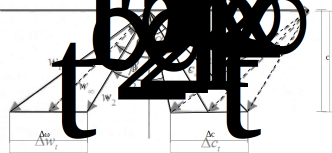
\includegraphics[width=\textwidth]{fig/SchiereCompr.pdf}
\caption{Schiere in movimento (compressore)}
\label{fig:SchiereCompr}
\end{figure}
Posso quindi calcolare la forza tangenziale data dalla variazione delle velocità relative tra ingresso e uscita.
\begin{align*}
\Delta c_t = c_{2t} - c_{1t} = \omega_{1t} - \omega_{2t} = |\Delta \omega_t |
\end{align*}
\begin{equation}
F_t = s \rho c_a (\omega_{1t} - \omega_{2t})
\end{equation}

Partendo dalle relazioni di potenza, portata in massa e forza tangenziale definisco il lavoro unitario.
\begin{equation}
\begin{cases}
P=F_t \cdot u\\
\dot{m} = \rho s c_a\\
F_t = c_F \cfrac{1}{2} \rho c \omega_{\infty}^2 = \cfrac{c_F \cfrac{1}{2} \rho c c_a^2}{\cos^2 \beta_{\infty}}
\end{cases}
\Rightarrow
L_u = \cfrac{F_t \cdot u}{\rho s c_a}
\end{equation}
Ottenendo infine
\begin{equation}
L_u = \cfrac{c_F \delta}{2 \cos^2 \beta_{\infty}} \cdot c_a \cdot u
\end{equation}
Sostituendo la relazione della forza tangenziale ottengo il lavoro unitario in funzione del coefficiente di forza, della solidità della schiera della velocità assiale e periferica. 

Con questa espressione si può ora adimensionalizzare il lavoro
\begin{equation}
\begin{cases}
\lambda = \cfrac{L_u}{\omega ^2 D^2} = \cfrac{L_u}{4 u^2}\\
\phi = \cfrac{Q}{\omega D^3} \propto \cfrac{c_a}{u} \\
\lambda = \cfrac{c_F \delta}{8 \cos^2 \beta_{\infty}} \cdot \cfrac{c_a}{u} = \cfrac{c_F \delta}{8 \cos^2 \beta_{\infty}} \cdot \phi
\end{cases}
\end{equation}
L'ultima espressione rappresenta la cifra di funzionamento della macchina in quanto ovviamente il lavoro viene fatto esclusivamente dalle parti rotoriche.

Si può quindi scrivere il rendimento isoentropico sia nel caso di compressione che di espansione. 

\begin{multicols}{2}
Compressione
\begin{equation}
\eta_{is} = \cfrac{L_u - \cfrac{\Delta p_0}{\rho}}{L_u} = 1- \cfrac{\cfrac{\Delta p_0}{\rho}}{L_u}
\end{equation}
\break
Espansione
\begin{equation}
\eta_{is} = \cfrac{L_u}{L_u + \cfrac{\Delta p_0}{\rho}} = \cfrac{1}{1+\cfrac{\cfrac{\Delta p_0}{\rho}}{L_u}}
\end{equation}
\end{multicols}

Utilizzando le relazioni note
\begin{align*}
\begin{cases}
\Delta p_0 = y \cfrac{1}{2} \rho \omega_2^2\\
L_u = \cfrac{c_F \delta}{2 \cos^2 \beta_{\infty}} \cdot c_a \cdot u\\
\omega_2 = \cfrac{c_a}{\cos \beta_2}\\
\phi = \cfrac{c_a}{u}
\end{cases}
\end{align*}
Si ottengono le espressioni
\begin{multicols}{2}
Compressione
\begin{equation}
\eta_{is} = 1- \cfrac{y}{c_F} \cdot  \cfrac{cos^2 \beta_{\infty}}{\delta \cos^2 \beta_2} \cdot \phi
\end{equation}
\break
Espansione
\begin{equation}
\eta_{is} = \cfrac{1}{1+\cfrac{y}{c_F} \cdot \cfrac{\cos^2 \beta_{\infty}}{\delta \cos^2 \beta_2} \cdot \phi}
\end{equation}
\end{multicols}
Ora vediamo cosa succede mettendo assime parte statorica e parte rotorica. Il rendimento di uno stadio assumerà l'espressione
\begin{equation}
\Delta p_0 = \Delta p_{0,stat} + \Delta p_{0,rot}
\end{equation}
\section{Equilibrio radiale}
\begin{figure}
\centering
  \includegraphics[width=\textwidth]{fig/ReticoloComp.pdf}
\caption{Reticolo di calcolo quasi-3D per un compressore assiale bistadio}
\label{fig:ReticoloComp}
\end{figure}
\begin{figure}
\centering
  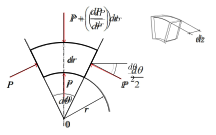
\includegraphics[width=.6\textwidth]{fig/concio.pdf}
\caption{Equilibrio radiale}
\label{fig:concio}
\end{figure}
Con questo abbiamo trattato cosa succede nell'attraversamento della schiera in termini macroscopici. Abbiamo già detto che per effettuare queste considerazioni bisogna partire dal presupposto che non vi sia un deflusso significativo in direzione radiale.
Devo assicurarmi che non vi sia trasmissione di forze tra sezioni circolari della macchina.

Si consideri l'elementino di fluido $dz - d\theta$ su cui agiscono le forze di pressione. 
Si calcoli l'equilibrio delle forze
\begin{equation}
\left( p + \cfrac{dp}{dr} dr \right) (r + dr) d \theta dz + pr d \theta dz -2p dr dz \sin \frac{d \theta}{2} = r \frac{dp}{dr} dr d \theta dz
\end{equation}
Linearizzando e trascurando i termini del secondo ordine si ottiene un termine che sarà equilibrato dalle forze centrifughe agenti sull'elemento. Perchè il moto non abbia componenti radiali deve quindi accadere che
\begin{equation}
\rho r d \theta dr dz \cdot \frac{V_t^2}{r} = r \frac{dp}{dr} dr d \theta dz\Rightarrow \cfrac{1}{\rho} \cfrac{dp}{dr} = \frac{V_t^2}{r}
\label{eq:EquilibrioRad}
\end{equation}

\subsection{Termodinamica}
Vediamo cosa succede da un punto di vista termodinamico.
Scriviamo l'entalpia di ristagno considerando che $V_r = 0$
\begin{equation}
h_0 = h + \cfrac{V^2}{2} = h + \cfrac{1}{2}(V_t^2 + V_a^2)
\end{equation}
Posso ora differenziare lungo il raggio ottenendo
\begin{equation}
\frac{dh_0}{dr} = \frac{dh}{dr} + V_t \frac{V_t}{dr} + V_a \frac{dV_a}{dr}
\label{eq:EntalpiaDiff}
\end{equation}
Considero ora il primo principio della termodinamica nella seguente forma
\begin{equation}
Tds = dh - \cfrac{1}{\rho} dp
\label{eq:PrimoPrinc}
\end{equation}
Mettendo assieme le equazioni \ref{eq:EntalpiaDiff} e \ref{eq:PrimoPrinc} ottengo
\begin{equation}
\frac{dh_0}{dr} = T \frac{ds}{dr} + \frac{1}{\rho} \frac{dp}{dr} + V_t \frac{dV_t}{dr} + V_a \frac{dV_a}{dr}
\end{equation}
Considerando poi l'equazione \ref{eq:EquilibrioRad} si ottiene
\begin{equation}
\frac{dh_0}{dr} = T \frac{ds}{dr} + \frac{V_t^2}{r} + V_t \frac{dV_t}{dr} + V_a \frac{dV_a}{dr}
\end{equation}
Ottengo un'espressione in cui non ho più una pressione ma solo i valori delle velocità, entalpia ed entropia al variare del raggio.
Ora posso scrivere l'equazione complessiva che rappresenta il legame da imporre per avere un flusso bidimensionale.
\begin{equation}
\boxed{ \frac{dh_0}{dr} - T\frac{ds}{dr} = V_a \frac{dV_a}{dr} + \frac{V_t}{r} \frac{d}{dr}(V_t \cdot r)}
\end{equation}
Questa equazione ci consente di affrontare due problematiche tipiche della progettazione delle macchine:
\begin{enumerate}
\item Problema diretto (o problema di verifica): nota la geometria di una macchina e la distribuzione radiale dell'angolo $\alpha_{\infty}$, determinare la distrubuzione radiale di tutte le grandezza del flusso e termidinamiche;
\item Problema inverso (o problema di progetto): assegnata una certa distribuzione di una grandezza termodinamica o fluidodinamica trovare qual'è la geometria della schiera che la realizza.
\end{enumerate}
\subsection{Ipotesi semplificative}
Posso fare un'ulteriore osservazione che semplifica la vita in fase di progettazione preliminare. Impongo
\begin{equation}
\begin{cases}
\cfrac{dh_0}{dr} = 0\\
\cfrac{ds}{dr} = 0
\end{cases}
\end{equation}
Ho imposto che $h_0$ e la dissipazione siano costanti lungo il raggio
In questo modo ottengo la relazione semplificata
\begin{equation}
\boxed{ V_a \frac{d V_a}{dr} + \frac{V_t}{r} \frac{d}{dr}(V_t \cdot r) = 0}
\label{eq:EquilibrioRadSemp}
\end{equation}
\section{Condizione di vortice libero}
Queste due osservazioni sono abbastanza realistiche. 
Facendo queste assunzioni sulle distribuzioni delle velocità tangenziali posso fare delle osservazioni sulle velocità assiali. 
Ad esempio posso costruire la macchina imponendo le condizioni di vortice libero, una delle tipiche condizioni imposte tra $V_a$ e $V_t$ ($V_t \cdot r = cost.$).
Questo significa che considerando un mantello $i$ generico.
\begin{equation}
V_t \cdot r = V_{ti} \cdot r_i \Rightarrow V_a = cost.
\end{equation}
Imponendo queste condizioni si ottiene una velocità assiale costante lungo il raggio (vedi Eq. \ref{eq:EquilibrioRadSemp}). Vediamo cosa succede dal punto di vista dell'entalpia considerando il rapporto tra una sezione generica e una sezione $i$. Sapendo che $h_0 = cost.$ si scrive
\begin{equation}
h + \frac{V^2}{2} = h_i + \frac{V_i^2}{2} \Rightarrow h = h_i	+ \frac{V_i^2 - V^2}{2}
\end{equation}
E quindi
\begin{equation}
\frac{h}{h_i} = 1 + \frac{1}{2h_i} (V_{ti}^2-V_t^2 + \cancel{V_a^2} -\cancel{V_a^2}) = 1 + \frac{1}{2h_i} \left( 1- \frac{V_t^2}{V_{ti}^2} \right)
\label{eq:RappEnt}
\end{equation}
Ma facendo un'ulteriore, semplicissima considerazione
\begin{align*}
V_t \cdot r = V_{ti} \cdot r_i \Rightarrow \frac{V_t}{V_{ti}} = \frac{r_i}{r}
\end{align*}
Posso scrivere la \ref{eq:RappEnt} nel modo seguente
\begin{equation}
\boxed{ \frac{h}{h_i} = 1 + \frac{1}{2h_i} \bigg(1 -  \left( \frac{r_i}{r}\right)^2 \bigg)}
\end{equation}
Rimanipolandola ulteriormente posso scriverla nella forma
\begin{equation}
\frac{h}{h_i} = 1 + \frac{\gamma -1}{2} M_{ti}^2 \bigg(1 -  \left( \frac{r_i}{r}\right)^2 \bigg) 
\end{equation}
Si possono ora diagrammare nelle condizioni di vortice libero tutte le espressini utili a livello termodinamico. Queste curve possono essere disegnate al variare del numero di Mach.
\begin{equation}
\begin{cases}
h = \cfrac{a ^ 2}{\gamma - 1} \\
M_{ti} = \cfrac{V_{ti}}{a_i}\\
\cfrac{h}{h_i} = 1 + \cfrac{\gamma -1}{2} M_{ti}^2 \bigg(1 -  \Big( \cfrac{r_i}{r}\Big)^2 \bigg)\\
\cfrac{p}{p_i} = \left( \cfrac{h}{h_i} \right)^{\frac{\gamma}{\gamma - 1}}
\end{cases}
\end{equation}
In Figura \ref{fig:VorticeLibero} è rappresentata la variazione di pressione al variare del numero di Mach.
\begin{figure}
\centering
  \includegraphics[width=.8\textwidth]{fig/VorticeLibero.pdf}
\caption{Pressione in funzione del raggio per un flusso a vortice libero}
\label{fig:VorticeLibero}
\end{figure}

\section{Vortice forzato}
Questo tipo di condizione non si realizza nella progettazione della macchina o nel suo funzionamento. Viene utilizzata per mitigare le problematiche relative al vortice libero introducendo una distribuzione di velocità diversa da quella prevista dal vortice libero. Condizione di vortice forzato:
\begin{equation}
\boxed{\frac{V_t}{r} = cost.}
\label{eq:VortForz}
\end{equation}
Questo significa che il deflusso della macchina si comporta effettivamente come un moto rigido, il rapporto tra velocità tangenziale e raggio si mantiene costante.
Si ricordano le equazioni di partenza, ovvero quella di equilibrio radiale e le ipotesi semplificative
\begin{align*}
\begin{cases}
\cfrac{dh_0}{dr} - T\cfrac{ds}{dr} = V_a \cfrac{dV_a}{dr} + \cfrac{V_t}{r} \cfrac{d}{dr}(V_t \cdot r)\\
\cfrac{dh_0}{dr} - T\cfrac{ds}{dr} = 0
\end{cases}
\end{align*}
Allora considerando la generica sezione $i$
\begin{align*}
\frac{V_t}{r} = \frac{V_{ti}}{r_i} \Rightarrow V_t = V_{ti} \frac{r}{r_i}
\end{align*}
Introducendo questa legge e sostituendo a $V_{ti}$ si ottiene
\begin{align*}
\boxed{\frac{d}{dr}\bigg( \frac{V_a^2}{2} \bigg) + \frac{V_{ti}}{r_i} \frac{d}{dr} \bigg(\frac{V_{ti}}{r_i} r^2 \bigg) = 0}
\end{align*}
Si tratta di un'equazione differenziale del primo ordine, risolvibile analiticamente. Infatti
\begin{equation}
\frac{d}{dr} \bigg( \frac{V_a^2}{2} \bigg) = -2 \bigg( \frac{V_{ti}}{r_i} \bigg) ^2 \cdot r
\Rightarrow
\bigg( \frac{V_a^2}{2} \bigg) = -2 V_{ti}^2 \bigg(\frac{r}{r_i} \bigg)^2 +C
\label{eq:SolCost}
\end{equation}
Devo andare allora a determinare la costante $C$. Posso dire che nella sezione i-esima la velocità assiale e raggio avranno il valore corrispondente.
\begin{align*}
\begin{cases}
V_a=V_{ai}\\
r=r_i
\end{cases}
\Rightarrow
C = \frac{V_{ai}^2}{2} + V_{ti}^2
\end{align*}
Sapendo che 
\begin{align*}
\frac{V_{ti}}{V_{ai}} = \tan \alpha_i
\end{align*}
Posso scrivere la \ref{eq:SolCost} nella forma completa
\begin{equation}
\boxed{ \bigg( \frac{V_a}{V_{ai}} \bigg)^2 = 1- 2 \tan^2 \alpha_i \bigg[ \bigg( \frac{r}{r_i} \bigg)^2 -1 \bigg] }
\label{eq:RappVol}
\end{equation}
Posso proseguire e andare a determinare anche l'andamento dell'entalpia in funzione del raggio.
Scrivo l'entalpia totale
\begin{align*}
h = h_i \frac{V_i^2 - V^2}{2}
\end{align*}
\begin{align*}
\frac{h}{h_i} = 1+ \frac{1}{2 h_i} (V_{ti}^2 - V_t^2 + V_{ai}^2 -V_a^2)
\end{align*}
Utilizzando poi la \ref{eq:VortForz} e raccogliendo i termini $V_{ti}$ e $V_{ai}$ ottengo
\begin{equation}
\boxed{ \frac{h}{h_i} = 1+ \frac{V_{ti}^2}{2 h_i} \bigg[ 1- \bigg( \frac{V_t}{V_{ti}} \bigg)^2 \bigg] + \frac{V_{ai}^2}{2 h_i} \bigg[ 1- \bigg( \frac{V_a}{V_{ai}} \bigg)^2 \bigg] }
\end{equation}
Posso fare delle ulteriori condsiderazioni ricordando la \ref{eq:RappVol} e le seguenti espressioni
\begin{align*}
\begin{cases}
\cfrac{V_t}{V_{ti}} = \cfrac{r}{r_i}\\
\cfrac{V_{ti}}{V_{ai}} \tan \alpha_i
\end{cases}
\end{align*}
Con alcuni passaggi algebrici si perviene a
\begin{equation}
\boxed{ \frac{h}{h_i} = 1+ \frac{V_{ti}^2}{2h_i} \bigg[ \bigg( \frac{r}{r_i} \bigg)^2 -1 \bigg] }
\end{equation}
Questo significa che a seconda dell'angolo di incidenza della palettatura, la distribuzione delle velocità assiali non è più uniforme lungo il raggio. Si vede chiaramente nel diagramma in Figura \ref{fig:TurboFan}.
\begin{figure}
\centering
  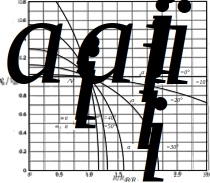
\includegraphics[width=.8\textwidth]{fig/VortForz.pdf}
\caption{Velocità assiale in funzione del raggio per un flusso a vortice forzato}
\label{fig:TurboFan}
\end{figure}
\begin{figure}
\centering
  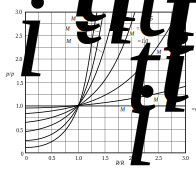
\includegraphics[width=.8\textwidth]{fig/PVortForz.pdf}
\caption{}
\label{fig:PVortForz}
\end{figure}
Naturalmente si può ricavare l'andamento delle pressioni e delle entalpie (Figura \ref{fig:PVortForz}). Ricordando che
\begin{equation}
\frac{p}{p_i} = \frac{h}{h_i}^{\frac{k}{k-1}}
\end{equation}
Allora
\begin{equation}
\frac{h}{h_i} = 1 + \frac{k-1}{2} M_{ti}^2 \bigg[ \bigg(\frac{r}{r_i} \bigg)^2-1 \bigg]
\end{equation}
L'entalpia varia con il raggio in maniera quadratica con una costante che dipende dal numero di Mach tangenziale. Si vede che a raggio $0$ le pressioni non sono nulle (al contrario del caso di vortice libero). Sebbene non faremo mai una macchina con vortice forzato sappiamo che nel caso il diametro all'albero sia particolarmente ridotto possiamo utilizzare una distribuzione diversa dal vortice libero. 

\subsection{A valle del vortice forzato}
Cosa succede però a valle della palettatura dopo aver attraversato un vortice forzato? 
Abbiamo imposto a valle la condizione di entalpia totale costante al variare del raggio
\begin{align*}
\frac{dh_{01}}{dr} = 0
\end{align*}
\begin{multicols}{2}
Sezione 1
\begin{align*}
\begin{cases}
h_{01} = cost.\\
V_{t1} = K_1 \cdot r
\end{cases}
\end{align*}
\break
Sezione 2
\begin{align*}
V_{t2} = K_2 \cdot r
\end{align*}
\end{multicols}
Possiamo calcolare il lavoro scambiato come differenza di entalpia totale
\begin{align*}
\begin{split}
h_{02} - h_{01} &= u (V_{t2} - V_{t1} ) = \omega r (K_2 r - K_1 r) \\
&= \omega (K_2 - K_1) r^2 = \Delta h_{012}
\end{split}
\end{align*}
Ovvero $\Delta h \propto r^2 \Rightarrow h_{02} \neq  cost.$. Via via che attraverso la macchina, a differenza del raggio in cui mi trovo cambia il lavoro scambiato dalla macchina, una condizione pressocchè impossibile da mantenere.

Possiamo andare a vedere cosa succede calcolando il differenziale dell'entalpia rispetto al raggio
\begin{align*}
\begin{split}
\cfrac{d \Delta h_{012}}{dr} &= \cfrac{d ( h_{02}-h_{01})}{dr} = \cfrac{dh_{02}}{dr} = \\
&= V_a \cfrac{dV_a}{dr} + \cfrac{V_t}{r} \cfrac{d}{dr} (V_t \cdot r) = 2 \omega (K_2 - K_1) r = \\
&= \cfrac{d}{dr} \bigg( \cfrac{V_{a2}^2}{2} \bigg) + K_2 \cfrac{d}{dr} (K_2 r^2)
\end{split}
\end{align*}
Anche questa è un'equazione differenziale lineare di primo ordine, posso risolverla
\begin{align*}
V_{a2}^2 = -2 \left[ K_2^2 - \omega \left( K_2 - K_1 \right) \right] r^2 + C
\end{align*}
La costante la calcolo integrando su tutta la sezione la portata in massa
\begin{align*}
\frac{\dot{m}}{2 \pi \rho} = \int_{rh}^{rs} V_{a1} r dr = \int_{rh}^{rs} V_{a2} r dr
\end{align*}
\begin{figure}[h]
\centering
  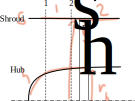
\includegraphics[width=.4\textwidth]{fig/HubShroud.pdf}
\caption{}
\label{fig:hubshroud}
\end{figure}
La portata entrante nella sezione uno deve essere uguale alla portata che entra nella sezione 2 (integrale da r-hub a r-shroud in Figura \ref{fig:hubshroud}).

\section{Vortice generico}
Spesso nella progettazione delle macchine assiali si usa una soluzione mista tra vortice libero e forzato. Si parla di vortice generico:
\begin{equation}
\begin{cases}
V_{t1} = a \cdot r^n - \frac{b}{r}\\
V_{t2} = a \cdot r^n + \frac{b}{r}
\end{cases}
\end{equation}
Definizioni:
\begin{itemize}
\item $n=0$: zero power blending
\item $n=1$: fast power blending
\end{itemize}
Il lavoro effettuato vale quindi 
\begin{equation}
L_u = h_{02} - h_{01} = u \left( V_{t2} - V_{t1} \right) = 2 \cdot b \cdot \omega
\end{equation}
Per $n=1$ ho una palettatura a grado di reazione costante, posso scrivere
\begin{align*}
R = 1 - \frac{V_2^2 - V_1^2}{2 L_u} = 1 - \frac{V_{t2}^2 + \cancel{V_{a2}^2} - V_{t1}^2 - \cancel{V_{a2}^2}}{2 L_u}
\end{align*}
Considerando $V_{a2} \simeq V_{a1}$, non è del tutto vero ma assumiamo la differenza piccola
\begin{align*}
R = 1 - \frac{\cancel{\left( V_{t2} - V_{t1} \right)} \left( V_{t2}+ V_{t1} \right)}{2 u \cancel{\left( V_{t2}- V_{t1} \right)}} = 1- \frac{\left( V_{t2}+ V_{t1} \right)}{2 u} = 1-\frac{a}{\omega} = cost.
\end{align*}
Ho dimostrato il grado di reazione costante.

\subsection{Angolo di palettatura costante}
Immagino di voler costruire una macchina con angolo di palettatura costante, significa che il bordo di attacco è rettilineo e solo la coda cambia l'angolo.
\begin{align*}
\frac{V_t}{V_a} = \tan \alpha = cost.
\end{align*}
Ci si chiede dunque come variano $V_t$ e $V_a$ al variare di $r$ rispettando l'equilibrio radiale.
Si avrà
\begin{align*}
\frac{V}{V_i} = \frac{V_a}{V_{ai}} = \frac{V_t}{V_{ti}} = \bigg(\frac{r_i}{r} \bigg)^{\sin \alpha}
\end{align*}
Con le solite ipotesi semplificative si ottiene
\begin{equation}
\frac{d}{dr} \bigg(\frac{V_a^2}{2} \bigg) + \frac{V_t}{r} \frac{d(rV_t}{dr} = 0
\end{equation}
Sapendo inoltre che
\begin{align*}
\begin{cases}
V_a = V \cos \alpha\\
V_t = V \sin \alpha
\end{cases}
\end{align*}
e facendo le opportune sostituzioni si perviene a
\begin{equation}
\boxed{\frac{dV}{dr} + \frac{V}{r} \sin^2 \alpha = 0}
\end{equation}
L'equazione differenziale è leggermente più complessa. La soluzione generica è di tipo esponenziale e bisogna sempre andare a determinare la costante generica. Si perviene alla seguente espressione.
\begin{align*}
y' + \phi(x)y + \psi(x) = 0 
\end{align*}
\begin{align*}
y = e^{-\int \phi(x)dx} \bigg[ C- \int \psi(x) e^{\int \phi(x)dx} dx \bigg] 
\end{align*}
In questo caso abbiamo $\phi(x) = 0$
\begin{align*}
V = e^{-\int \frac{\sin^2 \alpha}{r}dr}\cdot C = r^{-\sin^2 \alpha} \cdot C
\end{align*}
Sappiamo poi che per $r=r_i,\; V=V_i$ allora
\begin{align*}
C = \frac{V_i}{r_i^{-\sin^2 \alpha}}
\end{align*}
\begin{equation}
\boxed{ \frac{h}{h_i} =  1+ \frac{V_{ti}^2}{2 h_i \sin^2 \alpha} \bigg[1- \bigg(\frac{r_i}{r} \bigg) ^{2 \sin^2 \alpha} \bigg]}
\end{equation}
Si tratta di una soluzione adottata per le macchine a vapore che possiedono delle palettature molto massicce, si ottiene un andamento delle velocità assiali come in Figura \ref{fig:AngPalCost}. Questa è una distribuzione che non ha limiti teorici, si può sempre fare una macchina a bordo d'ingresso rettilineo. Rappresenta un caso intermedio tra un vortice libero e un vortice forzato.
\begin{figure}
\centering
  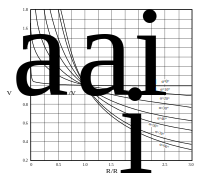
\includegraphics[width=.8\textwidth]{fig/AngPalCost.pdf}
\caption{}
\label{fig:AngPalCost}
\end{figure}
\begin{figure}
\centering
  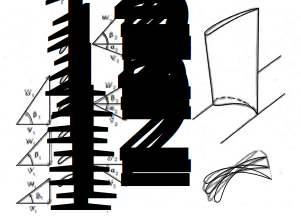
\includegraphics[width=.8\textwidth]{fig/TurboFan.pdf}
\caption{Profili e triangoli delle velocià per un rotore di turbo fan a vortice libero ($r_{TIP}/r_{HUB} =2$)}
\label{fig:TurboFan}
\end{figure}

\begin{figure}
\centering
  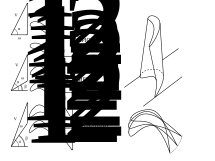
\includegraphics[width=.8\textwidth]{fig/TurbVortLib.pdf}
\caption{Profili e triangoli delle velocià per un rotore di uno stadio di bassa pressione di turbina a vapore o a gas ($r_{TIP}/r_{HUB} =1.4$)}
\label{fig:TurbVortLib}
\end{figure}

\begin{equation}
\Delta i_s = i_s - i_{s(s/c=0.75)}
\end{equation}
\begin{equation}
\frac{\alpha_1}{\alpha_1 (s/c = 0.75)}
\end{equation}
\begin{equation}
\frac{Y_p}{Y_{p(i=0)}}
\end{equation}